\section{Thực nghiệm phân loại nút trên Cora}
\subsection{Dữ liệu và nguồn gốc}
Cora biểu diễn các bài báo khoa học bằng các đặc trưng từ vựng và quan hệ trích dẫn. Mỗi dòng trong \path{cora.content} gồm mã bài báo, 1.433 biến nhị phân và một trong bảy nhãn chủ đề. Tệp \path{cora.cites} liệt kê các cặp trích dẫn. Dữ liệu được tải từ kho \texttt{tkipf/pygcn}, là kho mã tham chiếu của tác giả GCN; các tệp được đọc ở dạng văn bản và lưu mã băm SHA-256 để kiểm tra phiên bản.
\productlink{Nguồn dữ liệu Cora}{https://github.com/tkipf/pygcn/tree/master/data/cora}
Bộ dữ liệu có 2.708 nút và 5.429 dòng trích dẫn. Sau khi gộp các liên kết trùng, đối xứng hóa và bỏ cạnh tự nối ban đầu, đồ thị có 5278 cạnh vô hướng. Cạnh tự nối được thêm lại khi tính toán để mỗi nút giữ thông tin của chính nó. Nhãn là chủ đề của bài báo, không phải nhãn bệnh.

\subsection{Phép chia và giả thiết đánh giá}
Với seed 254, chọn ngẫu nhiên 20 nút trong mỗi lớp làm tập huấn luyện, tổng cộng 140 nút. Các nút còn lại được hoán vị; 500 nút đầu dùng cho validation, 1.000 nút tiếp theo dùng cho test, 1.068 nút còn lại không dùng nhãn trong tối ưu hoặc chọn checkpoint. Đây là phép chia riêng có phân tầng, không phải phép chia Planetoid chuẩn. Mã bài báo và vai trò từng nút được lưu trong \path{results/cora/split.csv}.

Thiết lập là transductive: đặc trưng và cấu trúc của toàn bộ đồ thị có mặt khi truyền thông điệp, nhưng gradient chỉ dùng nhãn của 140 nút train. Validation chỉ dùng để chọn checkpoint có cross-entropy nhỏ nhất trong ngân sách 200 epoch. Nhãn test chỉ dùng sau khi hoàn tất lựa chọn. Ba seed 254, 255 và 256 thay đổi khởi tạo trọng số; phép chia dữ liệu giữ cố định để tách biến thiên do tối ưu khỏi biến thiên do lấy mẫu.

\subsection{GCN và mô hình đối chứng}
Hai mô hình cùng có một tầng ẩn 16 chiều, ReLU và đầu ra softmax bảy lớp. GCN dùng phép truyền thông điệp ở cả hai tầng:
\[
Z=\operatorname{softmax}\left(\widehat A\operatorname{ReLU}(\widehat A XW_0)W_1\right).
\]
MLP thay $\widehat A$ bằng ma trận đơn vị nên chỉ sử dụng đặc trưng của từng bài báo. Các hàng của $X$ được chuẩn hóa theo tổng số từ xuất hiện; phép biến đổi này thực hiện độc lập trên từng nút và không sử dụng nhãn. Ma trận kề được chuẩn hóa đối xứng theo bậc.

Hàm mục tiêu gồm cross-entropy trên tập train và $\frac{\lambda}{2}\lVert W_0\rVert_F^2$, với $\lambda=5\times10^{-4}$. Cả hai mô hình dùng Adam, tốc độ học 0,01, $\beta_1=0,9$, $\beta_2=0,999$ và 200 epoch. Không dùng dropout, bias hoặc tìm kiếm siêu tham số trong thí nghiệm này. Các điều kiện đó giữ phép so sánh tập trung vào việc có hoặc không dùng cấu trúc đồ thị.

\subsection{Cài đặt và kiểm tra gradient}
Mã \path{scripts/train_cora.py} cài đặt lan truyền thuận và gradient bằng NumPy; SciPy lưu ma trận thưa. Nếu $S=\widehat AX$, $H=\operatorname{ReLU}(SW_0)$ và $D=\partial L/\partial Z_{\mathrm{logit}}$, ta có:
\[
\frac{\partial L}{\partial W_1}=(\widehat AH)^TD,\qquad
\frac{\partial L}{\partial W_0}=S^T\left[(\widehat A^TDW_1^T)\odot\mathbf1_{SW_0>0}\right]+\lambda W_0.
\]
Gradient được đối chiếu với sai phân trung tâm trên một đồ thị nhỏ trước khi huấn luyện. Sai số tuyệt đối lớn nhất nhỏ hơn $10^{-6}$. Kiểm tra này xác nhận phép đạo hàm trong điều kiện thử, không thay cho đánh giá độ chính xác trên Cora.
\section{Kết quả và phân tích}
\subsection{So sánh trên cùng tập kiểm tra}
\begin{table}[H]\centering\small\caption{GCN và MLP trên phép chia Cora cố định; mỗi mô hình chạy ba seed.}\label{tab:cora-results}
\begin{tabular}{lrrrr}\toprule Mô hình & Seed & Epoch chọn & Accuracy & Macro-F1\\\midrule
MLP & 254 & 200 & 0.5450 & 0.5400\\
MLP & 255 & 200 & 0.5500 & 0.5444\\
MLP & 256 & 200 & 0.5460 & 0.5351\\
GCN & 254 & 200 & 0.8050 & 0.7879\\
GCN & 255 & 200 & 0.8040 & 0.7895\\
GCN & 256 & 200 & 0.8020 & 0.7886\\
\bottomrule\end{tabular}\end{table}
Qua ba seed, accuracy của GCN là $0.8037\pm0.0015$, còn MLP là $0.5470\pm0.0026$. Macro-F1 tương ứng là $0.7887\pm0.0008$ và $0.5399\pm0.0046$. Dấu $\pm$ là độ lệch chuẩn mẫu giữa ba khởi tạo, không phải khoảng tin cậy.

Ở cả sáu lượt chạy, checkpoint được chọn tại epoch 200. Vì điểm validation còn cải thiện đến giới hạn ngân sách, không kết luận mô hình đã hội tụ hoàn toàn. So sánh hiện tại chỉ áp dụng cho cùng phép chia, kiến trúc và ngân sách học nêu trên; không dùng các số này để xếp hạng với kết quả công bố trên phép chia khác.
\begin{figure}[H]\centering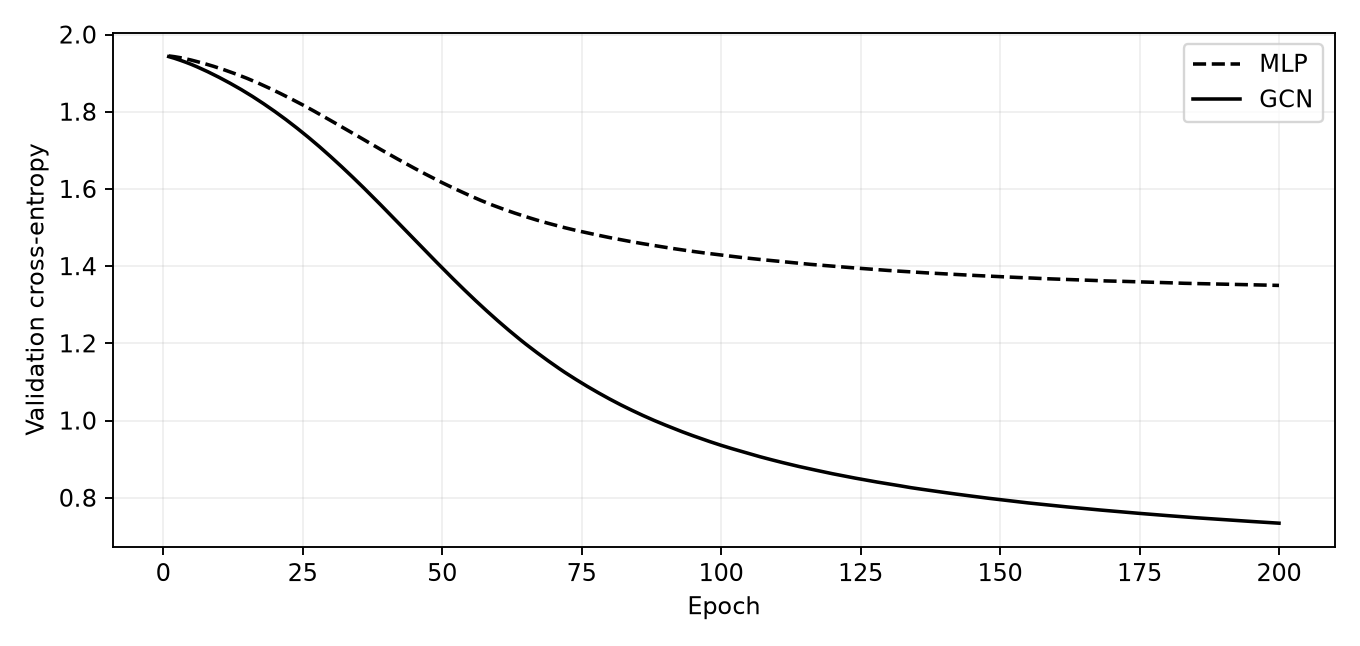
\includegraphics[width=.94\linewidth]{figures/cora-learning.png}\caption{Cross-entropy validation theo epoch của MLP và GCN, seed 254.}\end{figure}
\subsection{Phân bố lỗi theo chủ đề}
\begin{figure}[H]\centering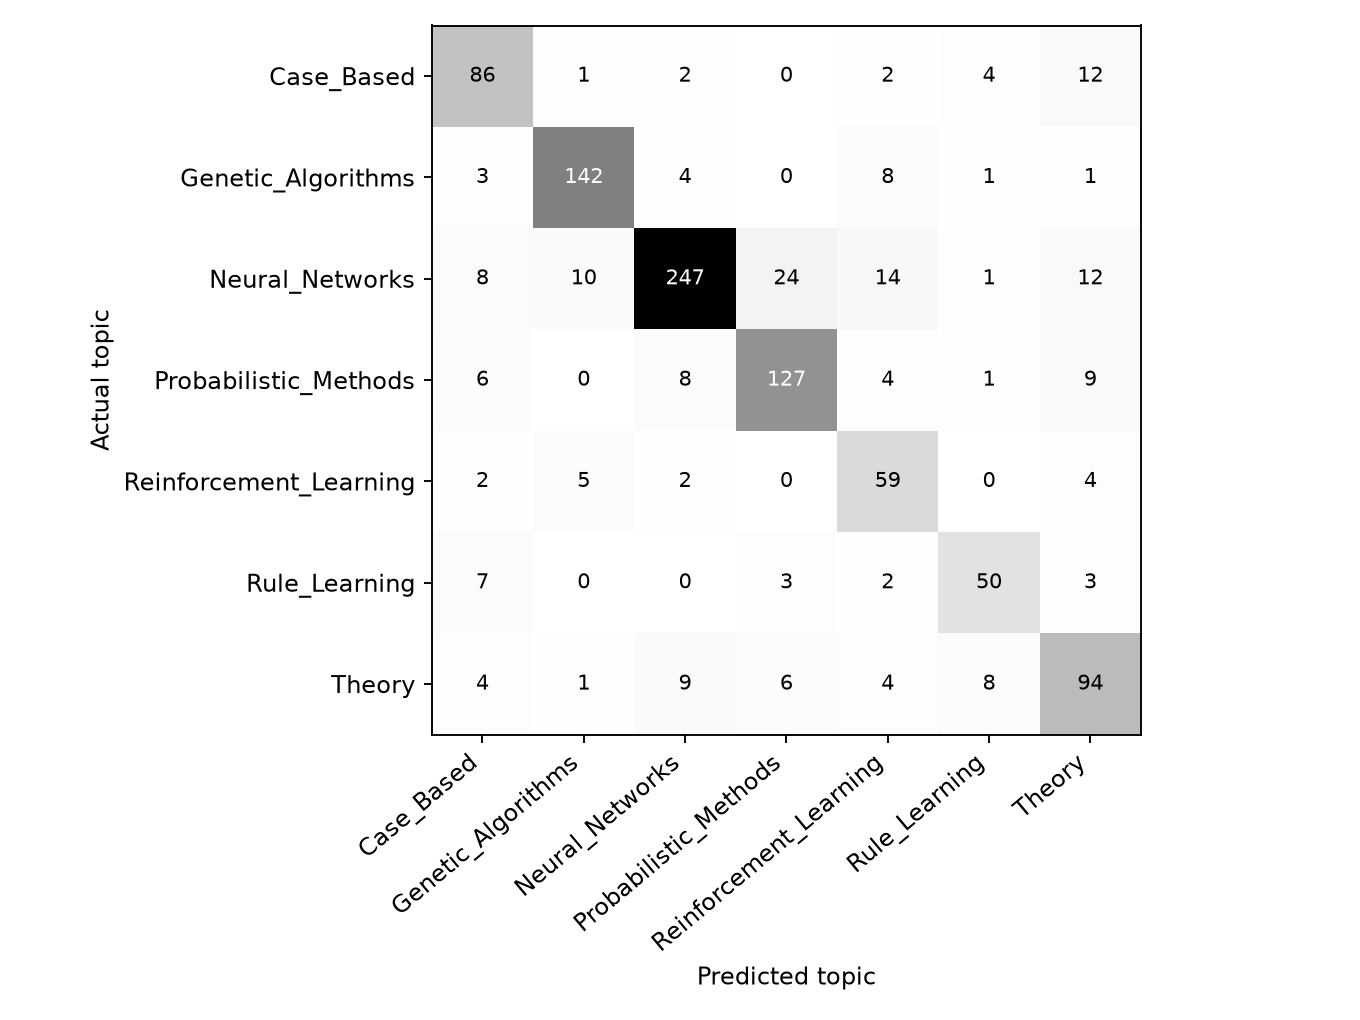
\includegraphics[width=.92\linewidth,height=.48\textheight,keepaspectratio]{figures/cora-confusion.png}\caption{Ma trận nhầm lẫn của GCN trên 1.000 nút test, seed 254.}\end{figure}
Ma trận nhầm lẫn bổ sung thông tin mà accuracy tổng thể không phản ánh. Các ô ngoài đường chéo cho thấy chủ đề nào bị lẫn với chủ đề khác; macro-F1 coi trọng từng lớp như nhau nên phù hợp khi số bài báo giữa các chủ đề khác nhau. Các liên kết trích dẫn giúp đưa thông tin từ bài báo liên quan vào biểu diễn, nhưng một trích dẫn không luôn nối hai bài thuộc cùng chủ đề.

\section{Khả năng tái lập và giới hạn}
\subsection{Mã nguồn và kết quả lưu}
\productlink{Mã thực nghiệm GCN}{https://github.com/jellalaz/He_Thong_Thong_Minh_Thay_Que/blob/main/scripts/train_cora.py}
Chạy \texttt{python scripts/train\_cora.py} sau khi cài các thư viện thực nghiệm. Chương trình tải hai tệp nguồn nếu chưa có, dựng phép chia, kiểm tra gradient, huấn luyện và xuất bảng kết quả. Thư mục \path{results/cora/} chứa mã băm dữ liệu, phép chia, dự đoán từng nút, đường học và trọng số \texttt{npz}. Hai hình trong chương được sinh trực tiếp từ kết quả đó.
\subsection{Phạm vi kết luận}
Ba seed chỉ đo ảnh hưởng khởi tạo trên một phép chia; muốn đánh giá ổn định theo dữ liệu phải dùng thêm nhiều phép chia. Đồ thị được đối xứng hóa nên không còn phân biệt chiều trích dẫn. MLP và GCN không được tìm siêu tham số riêng; kết quả vì vậy minh họa tác dụng của liên kết trong cấu hình đang xét, không chứng minh GCN luôn tốt hơn trên mọi đồ thị. Thí nghiệm Cora không đánh giá khả năng tư vấn y tế hoặc độ đúng của tri thức.
\section{Tiểu kết chương}
GCN mở rộng mạng nơ-ron từ các mẫu độc lập sang dữ liệu có liên kết thông qua phép tổng hợp lân cận. Thực nghiệm Cora cho thấy cấu trúc đồ thị có ích khi số nút được gán nhãn ít. Tuy nhiên, phép chia, hướng cạnh và cách lựa chọn checkpoint quyết định ý nghĩa của kết quả; các yếu tố này cần được công bố cùng chỉ số đánh giá.
